% This is samplepaper.tex, a sample chapter demonstrating the
% LLNCS macro package for Springer Computer Science proceedings;
% Version 2.20 of 2017/10/04
%
\documentclass[runningheads]{llncs}
%
\usepackage{lipsum}  
\usepackage{graphicx}
\usepackage{booktabs}
% Used for displaying a sample figure. If possible, figure files should
% be included in EPS format.
%
% If you use the hyperref package, please uncomment the following line
% to display URLs in blue roman font according to Springer's eBook style:
% \renewcommand\UrlFont{\color{blue}\rmfamily}
% The following line is for merging abstracts into proceedings later:
% \documentclass[abstract-main.tex]{subfiles} 
\begin{document}
%
\title{How Long Should We Pronounce to Sound Native in Dutch?\\ The Correlation between VOT of /t/ and /d/ in Dutch Produced by Chinese Learners and the Foreign Accent Perception}
%
\titlerunning{How Long Should We Pronounce to Sound Native in Dutch?}
% If the paper title is too long for the running head, you can set
% an abbreviated paper title here
%
\author{Cantao Su\inst{1} \and
Chenyu Li\inst{1} \and
Weihao Jiang\inst{1} \and 
Yanhua Liao\inst{1} }
%
\authorrunning{Cantao Su, Chenyu Li, Weihao Jiang, Yanhua Liao}
% First names are abbreviated in the running head.
% If there are more than two authors, 'et al.' is used.
%
\institute{University of Groningen, Campus Frysl\^an}
%
\maketitle              % typeset the header of the contribution
%
%
%
\section*{Abstract}
\subsection*{Background}
It is relatively difficult for Chinese to speak Dutch natively. One of the reasons is that two consonants /t/ and /d/ very common in Dutch, exhibit notable distinctions from their Mandarin Chinese counterparts. In Mandarin, /t/ is an aspirated voiceless consonant, while /d/ is an unaspirated voiced consonant. In Dutch /t, d/ are typically articulated with the blade of the tongue forming a closure with a relatively large area of the alveolar ridge while /t/ is characterized by voiceless unaspiration, and /d/ is fully voiced.  /t/ is characterized by voiceless unaspiration, and /d/ is fully voiced. This phonemic contrast introduces a challenge for Mandarin speakers, who commonly encounter difficulty distinguishing between these two consonants in listening comprehension and struggle to articulate them distinctly in spoken Dutch. This challenge in learning Dutch poses a barrier to achieving a natural and native-like pronunciation, potentially resulting in miscommunications.

Simultaneously, as we delve into the investigation of consonantal features, Voice Onset Time (VOT) emerges as a pivotal metric. Therefore, bearing this in mind, we contemplate whether the VOT duration in the pronunciation of Dutch /t/ and /d/ by Chinese learners of Dutch influences their perceived foreign accent in speech.

Given the intricate phonetic landscape shaped by these differences, we hypothesized that VOT durations of the /t/ and /d/ consonants in Dutch produced by Chinese learners, which are significantly different from the range of VOTs from native speakers, would result in strong foreign accent perception rated by native speakers.



% the environments 'definition', 'lemma', 'proposition', 'corollary',
% 'remark', and 'example' are defined in the LLNCS documentclass as well.
%
\subsection*{Methods}
Our study investigates the potential correlation between Voice Onset Time (VOT) duration for the /t/ and /d/ consonants in Dutch, as produced by Chinese learners of Dutch, and their foreign accent perceived by Dutch native speakers. 

\subsubsection*{Participants:}
Ten Chinese participants (5 females and 5 males) with a proficiency level around A1 in Dutch, along with ten Dutch native speakers, were recruited for this experiment. 

\subsubsection*{Selection of Experimental Vocabulary:}
Two pairs of words ('later' with 'lader' and 'tak' with 'dak') were carefully chosen as the experimental vocabulary. These words were pronounced by all 20 participants in the same order, and their recordings were collected.

\subsubsection*{Rationale for Word Selection:}
The selection of these word pairs was guided by linguistic considerations to effectively isolate the impact of VOT duration while controlling for other linguistic factors:\cite{gabriel_vot_2016} \\
\underline{Similar Environment and Minimal Sound Variation:} The word pairs 'later' and 'lader' and 'tak' and 'dak' were chosen because they share the /t/ and /d/ consonants. This design ensures that the pronunciation environment for these consonants is consistent within each pair. By using these word pairs, we reduce variations in vowel quality, stress patterns, and syllable structures, enabling us to focus on VOT variations specific to the /t/ and /d/ sounds.\\
\underline{Natural Word Choices:} 'Later,' 'lader,' 'tak,' and 'dak' are common, everyday words in the Dutch language. This choice guarantees that the pronunciations by our participants reflect typical speech patterns.

\subsubsection*{Data Collection and Analysis:}
Recordings from all participants were meticulously analyzed, and VOT data were quantified using Praat. The collected data were then used to create box plots with Python, providing a visual representation of descriptive statistics. \cite{cho_phonological_2006}

To test and verify if the differences between the two datasets are statistically significant, we employed a t-test using the SciPy library in Python to calculate the respective t value and p value. The t-value represents the difference between the means of the two datasets while considering this difference relative to the variability (variance) of the data and the sample size. If the absolute value of the t-value is greater than 1.96, the difference can be considered significant. The p-value is a crucial output of the t-test. A lower p-value suggests a more significant difference. The difference is considered significant if the p-value is less than the significance level (often set at 0.05).
 
Subsequently, those with a noticeable difference were selected for further analysis in the subsequent phase of post perceptual survey.

\subsubsection*{Post Perceptual Survey:}
To examine the correlation between foreign accent perceived by native speakers and the VOT duration of the /t/ and /d/ consonants, a post-perceptual survey was conducted. Ten Dutch native speakers, randomly selected from the public, were asked to evaluate the foreign accent of the recorded pronunciations while listening through earphones. A 5-point Likert scale was utilized in the survey to obtain a nuanced assessment.

Next, we will use the VOT values of the Dutch speakers as the standard dataset. We will calculate the deviation of individual Chinese speakers' VOT values for the from the standard dataset. By comparing these deviation values, it can be determined which learner  is closer to the standard dataset in terms of VOT values. Smaller deviation values indicate smaller differences, so the learner with the smaller deviation is closer to the standard.\cite{van_alphen_acoustical_2004}

By using each Chinese speaker's VOT deviation as the independent variable and their accent perception scores as the dependent variable, a statistical graph is created to observe the relationship between VOT and accent perception.

\subsection*{Results}

\underline{Visualization of Comparison:}

To visualize the data distribution among VOT of /t/ and /d/ pronounced by native speaker and Chinese learner, box plots are created by python using matplotlib library. 
\begin{figure}
    \centering
    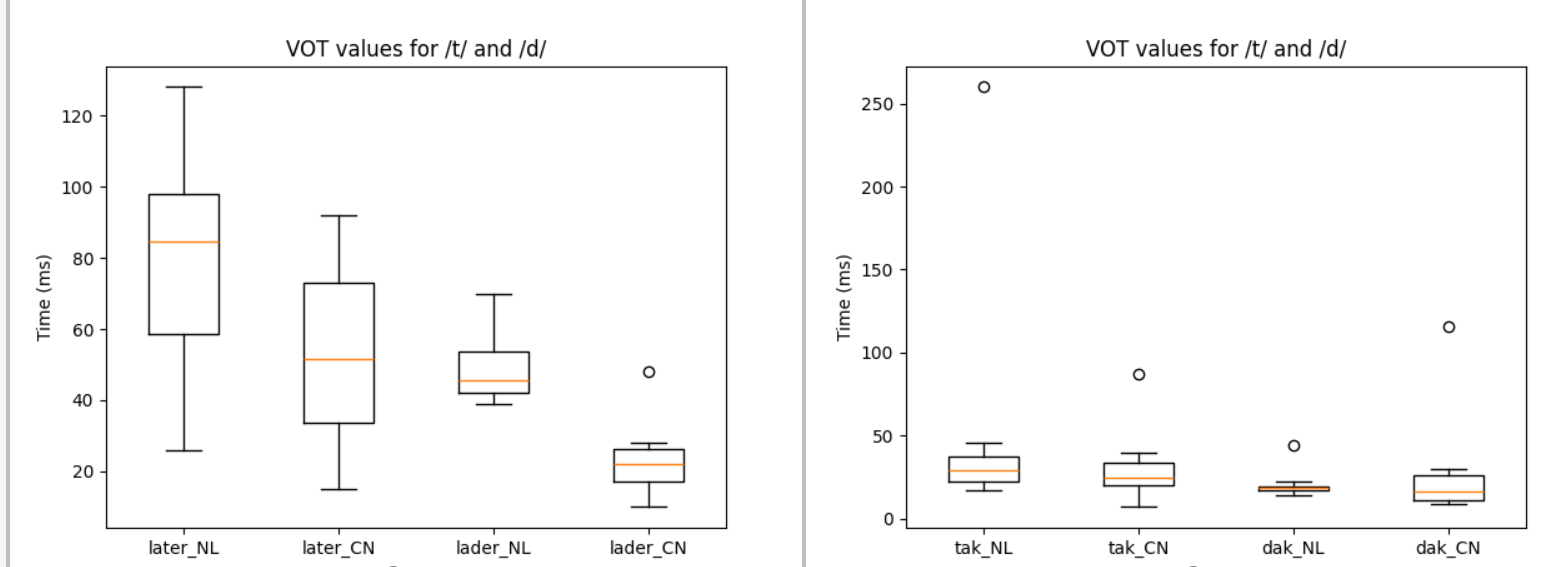
\includegraphics[width=1\textwidth]{Figure1.jpg}
    \caption{VOT values for /t/ and /d/ by Dutch native speaker and Chinese learner of Dutch}
\end{figure}

\underline{Statistical Testing:} see Table 1.
\begin{table}
	\centering
	\caption{Result of T-Test by VOT comparison between the native speakers and Chinese learners}
	\begin{tabular}{lcccc}
	\toprule
	& Tak & Dak & Later & Lader \\
	\midrule
	t-value & -0.223 & -0.588 & 2.073 & 5.664 \\
	p-value & 0.825 & 0.563 & 0.052 & $2.25 \times 10^{-5}$ \\
	\bottomrule
	\end{tabular}
\end{table}


\underline{Perceptual Survey:}

The survey results indicate that the ten Dutch interviewees were able to distinguish between native speakers and Chinese learners of Dutch by listening to the recordings. The average score for the Dutch native speaker was 4.5 points, while the average score for the Chinese learners was 2.3 points. The highest score for the Chinese learners was 3 points, and the lowest score was 1.8 points. \cite{van_sluis_acoustic_nodate}
The scores for the perception of foreign accents by Chinese speakers in relation to VOT of the deviation from native speakers are shown in the following table:
\begin{figure}
    \centering
    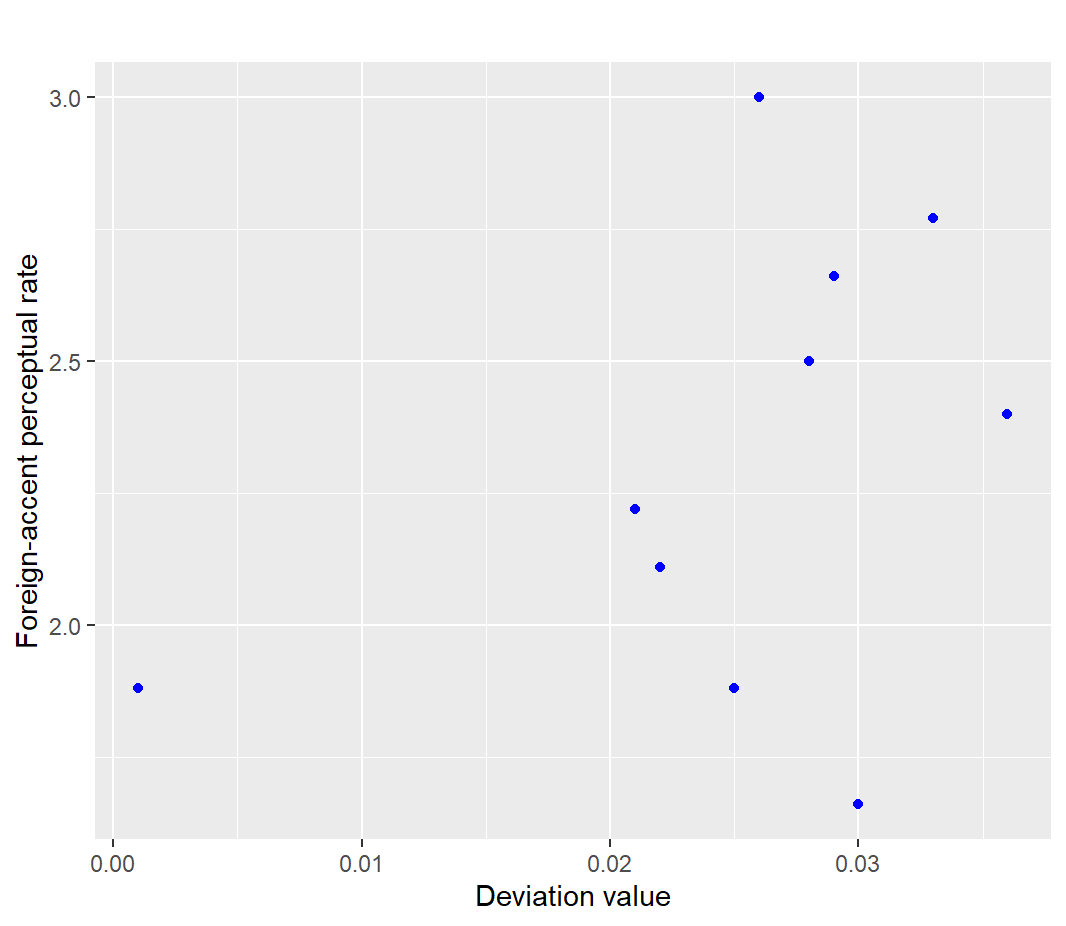
\includegraphics[width=0.8\textwidth]{Figure2.jpg}
    \caption{VOT deviation and their foreign accent perception scores}
\end{figure}

\subsection*{Discussion}
The objective of this experiment is to investigate the relationship between the speech feature Voice Onset Time (VOT) and foreign accent perception. Our research results demonstrate that A1-level Chinese learners participating in this experiment are perceived to have a distinct foreign accent. In our analysis of VOT, we discovered an intriguing phenomenon.

Our experimental data indicate that the most significant differences in VOT data between Chinese learners of Dutch and native Dutch speakers are observed in the production of voiced plosives in the mid-position. It is interesting that the experimental results show that A1-level Chinese learners of Dutch display similar patterns to Dutch children in their ability to distinguish /t/ and /d/. Acquisition of the phonological contrast between these two consonants is reported to be difficult for Dutch children (Gillis 2004). Van der Feest (2004) observed that Dutch children acquire the contrast between voiced and voiceless stops in pronunciation relatively late, around the age of 2.6 years. Voiceless stops are produced first and more accurately than their voiced counterparts in both word onset and word medial position (Beers 1995, Van der Feest 2007). \cite{hanssen_t-bias_2015}

Initially, our intuition led us to believe that if the VOT of /t/ and /d/ among Chinese learners closely approximated that of native Dutch speakers, or fell within the VOT range of native Dutch speakers, the pronunciation of /t/ and /d/ by Chinese learners would be perceived as more native-like. In other words, the difference in VOT compared to that of native speakers would be positively correlated with the perception of a foreign accent.

However, during our accent perception survey, we found no apparent linear correlation between subjective accent severity ratings and individual VOT deviation values. Some learners rated as more standard accent had high VOT deviation values from the range of the VOT of native speakers, while some rated as strong accented had low VOT deviation values. 

This result prompted us to contemplate the complexity and diversity of accent perception. Accent perception is influenced by a combination of various factors, including syllable stress, speech rhythm, grammar, and cultural elements. Consequently, VOT, while being an important speech feature, cannot fully explain the complexity of accent perception.


\subsection*{Conclusion}
In conclusion, the results of this experiment suggest that VOT is not the sole determinant of the foreign accent perception of Dutch consonants /t/ and /d/. While VOT is an important feature in phonetics, accent perception is influenced by multiple factors, including syllable stress, prosody, grammar, and cultural elements. The differences in accent perception between native Dutch speakers and Chinese learners of Dutch may be the result of a combination of various phonetic features and factors.

Based on the experimental data from our interviews with 10 native Dutch speakers and 10 Chinese learners of Dutch at the A1 level, we have concluded that there is no apparent linear correlation between VOT and the perception of a foreign accent, which suggests that VOT is not the sole determinant of the foreign accent perception of Dutch consonants /t/ and /d/. While VOT is an important feature in phonetics, accent perception is influenced by multiple factors, including syllable stress, prosody, grammar, and cultural elements.  However, we must acknowledge several limitations in this study.

Firstly, the sample size is relatively small, which might have restricted our ability to investigate more subtle relationships between VOT and accent perception. Future research is recommended to expand the sample size to better capture and understand potential correlations between VOT and accent perception.

Secondly, we suggest that future studies should rigorously control for source variables to reduce external factors' interference with accent perception. This includes a more comprehensive consideration of phonetic rhythm, grammar, cultural factors, and other elements that might affect accent perception.

In summary, while our study has provided preliminary insights into the relationship between VOT and accent perception, accent perception is a complex subjective process involving various factors. Future research should delve deeper into the mechanisms of accent perception and gain a better understanding of VOT's role within it.


\keywords{VOT duration  \and Dutch consonants \and Foreign accent perception \and Phonetic features.}

\subsection*{Authors' contributions}
Cantao conducted literature review, gathering and organizing relevant research to establish a strong theoretical foundation. He also helped with the inclusion of proper references in the research report to maintain academic rigor. His responsibilities also cover formulating and justifying our research proposal and methodology, and writing the introduction and methodology sections of our experiment report,  language editing and LaTeX formatting. \\
Chenyu's responsibilities included gathering and organizing literature, designing the research proposal, and performing statistical analysis. She also created data visualizations and participated in discussions. She crafted the result and conclusion sections of our report, synthesizing our findings and connecting them to our research objectives. \\
Weihao organized the questionnaire data, assisted the questionnaire survey, was responsible for the extraction of audio vot, the production of pictures and ppt with python and R languages, and participated in the discussion of abstract.\\
Yanhua was responsible for the extraction and analysis of VOT data, collecting recordings, contacting volunteers to do questionnaires, and participating in the discussion of abstract content.
%
% ---- Bibliography ----
%
% BibTeX users should specify bibliography style 'splncs04'.
% References will then be sorted and formatted in the correct style.
%
\bibliographystyle{refs-style}
\bibliography{refs}
%

\end{document}
